% TELOS Three-Tier Governance Flow
% Standalone compilable TikZ diagram
% Compile with: pdflatex fig1_three_tier_governance.tex

\documentclass[border=10pt]{standalone}
\usepackage{tikz}
\usetikzlibrary{positioning, arrows.meta}

\begin{document}
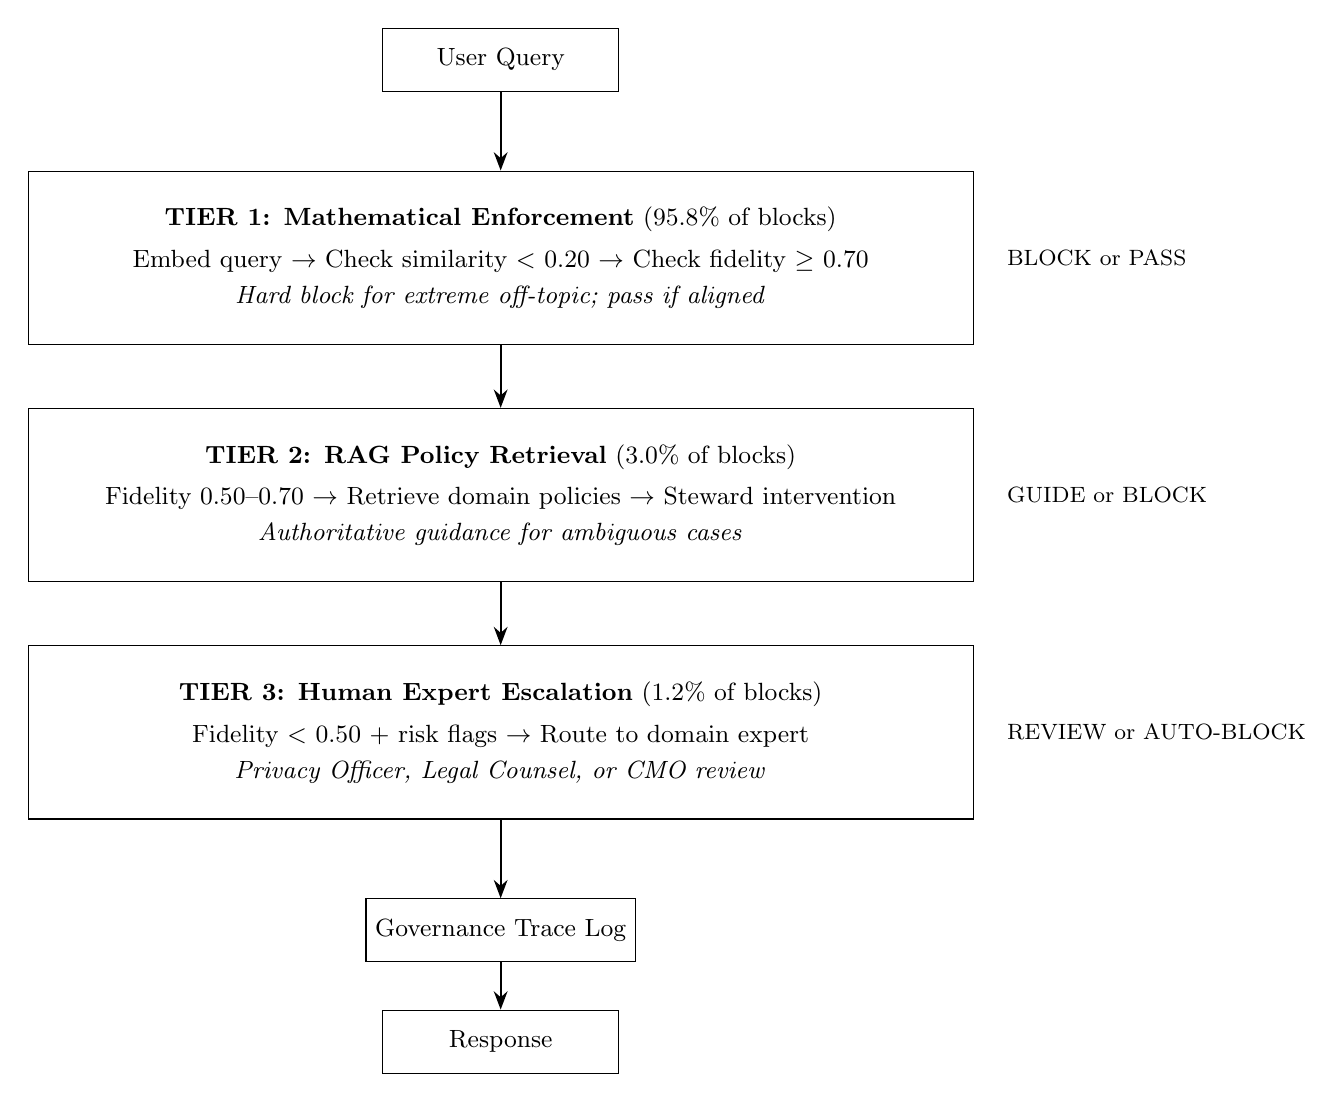
\begin{tikzpicture}[
    >=Stealth,
    node distance=1cm,
    box/.style={
        rectangle,
        draw,
        minimum width=12cm,
        minimum height=2.2cm,
        align=center,
        font=\small
    },
    smallbox/.style={
        rectangle,
        draw,
        minimum width=3cm,
        minimum height=0.8cm,
        align=center,
        font=\small
    },
    arrow/.style={->, thick}
]

% Input
\node[smallbox] (input) {User Query};

% Tier 1
\node[box, below=1cm of input] (tier1) {
    \textbf{TIER 1: Mathematical Enforcement} (95.8\% of blocks)\\[4pt]
    Embed query $\rightarrow$ Check similarity $<$ 0.20 $\rightarrow$ Check fidelity $\geq$ 0.70\\[2pt]
    \textit{Hard block for extreme off-topic; pass if aligned}
};

% Tier 2
\node[box, below=0.8cm of tier1] (tier2) {
    \textbf{TIER 2: RAG Policy Retrieval} (3.0\% of blocks)\\[4pt]
    Fidelity 0.50--0.70 $\rightarrow$ Retrieve domain policies $\rightarrow$ Steward intervention\\[2pt]
    \textit{Authoritative guidance for ambiguous cases}
};

% Tier 3
\node[box, below=0.8cm of tier2] (tier3) {
    \textbf{TIER 3: Human Expert Escalation} (1.2\% of blocks)\\[4pt]
    Fidelity $<$ 0.50 + risk flags $\rightarrow$ Route to domain expert\\[2pt]
    \textit{Privacy Officer, Legal Counsel, or CMO review}
};

% Output
\node[smallbox, below=1cm of tier3] (trace) {Governance Trace Log};
\node[smallbox, below=0.6cm of trace] (output) {Response};

% Arrows - simple vertical flow
\draw[arrow] (input) -- (tier1);
\draw[arrow] (tier1) -- (tier2);
\draw[arrow] (tier2) -- (tier3);
\draw[arrow] (tier3) -- (trace);
\draw[arrow] (trace) -- (output);

% Side labels for outcomes
\node[font=\footnotesize, right=0.3cm of tier1.east, anchor=west] {BLOCK or PASS};
\node[font=\footnotesize, right=0.3cm of tier2.east, anchor=west] {GUIDE or BLOCK};
\node[font=\footnotesize, right=0.3cm of tier3.east, anchor=west] {REVIEW or AUTO-BLOCK};

\end{tikzpicture}
\end{document}
